\chapter{Clustering}
\nomenclature{Glossary term:}{Definition}

Often, we are not only interested in specific data points, but also in the relationships between those data points.
Cluster analysis refers to the grouping of data points into \emph{clusters} based on similar characteristics.
R has variety of libraries that support cluster analysis.
We will use \texttt{cluster.datasets} for this lesson, in which we will analyze clustering in data about crime rates in US cities. \cite{Novomestky}
\medskip

Here are some typical commands used in cluster analysis:

\begin{enumerate}
\item \texttt{scale}
\item \texttt{k.means.fit}
\item \texttt{attributes}
\item \texttt{wssplot}
\item \texttt{clusplot}
\item \texttt{dist}
\item \texttt{hclust}
\item \texttt{groups}
\item \texttt{rect.hclust}
\item \texttt{table}

\end{enumerate}


For this study, you will learn a basic framework for cluster analysis using two different methods, K-means and hierarchical clustering.
Each method produces a different type of cluster graph of the same data. 

\begin{itemize}

\item Your first task is to graph a set of data using the K-means clustering method.

\item Your second task is to graph a set of data using the hierarchical clustering method. 
 
\end{itemize}

\section{Building the Model}

You should begin by copying and pasting the teaching code into RStudio.
This will serve as a foundation upon which to build your code.
We have included comments to guide you as you complete the code by adding commands.
When you successfully complete the code, it should output two graphics, shown in figures \ref{fig:Kmeans} and \ref{fig:Tree}.

\subsection{Programming Hints}

\begin{enumerate}
 
\item Different datasets will often require different clustering methods.
Therefore, not all clustering methods will work (or at least, work well) for every dataset!
Be prepared to use a variety of clustering methods in the future.
\item When installing packages, install them in the ``console'' window of RStudio.
\item If a piece of code is indented in the teaching or student code, it must also be indented in the code that you write.
This is important!
 
\end{enumerate}

\section{Deliverable}

The final product that you create should consist of one K-means cluster graph composed of groups of data points embedded in ovals and one hierarchical tree plot. 

\section{Teaching Code}

\begin{lstlisting}
    
# Your Name
# Date
# Script name: dataset.R
# Objective of script
#
# set working directory where results will be saved
setwd("file location")
#
# install the necessary package and datasets, then read in library
install.packages("data package") 
# this particular step should be completed in the console window
library(data package)
data(dataset, package = 'data package') 
# "dataset" is the name that you choose to call your specific dataset 
head(dataset)
#
# now we will begin to complete the first objective
#
# begin by standardizing the variables
dataset <- scale(original.dataset.name[-1])
#
# this next piece of code is the K-means function, where the number
# # symbol denotes the number of cluster groups
k.means.fit <- kmeans(dataset, #)
#
# this code segment includes all of the outputs of the k.means.fit function
attributes((k.means.fit))
#
# this next piece of code denotes the centroids
k.means.fit$centers # a nice table should result
#
# this piece of code shows the clusters
k.means.fit$cluster
#
# this code string denotes the size of the clusters
k.means.fit$size
#
# now we will begin to complete the first objective
#
# load the cluster library
library(cluster)
#
# this next section of code creates the a cluster graph using the K-means method
clusplot(dataset, k.means.fit$cluster, main = "Name of Cluster Graph", color = TRUE, 
shade = TRUE, labels = 2, lines = 0) # look at those nice colorful ovals!
#
# this next line creates a confusion matrix which evaluates the performance of the clustering
table(dataset[,1],k.means.fit$cluster)
#
# Okay, now that you've mastered k-means clustering, 
# let's move on to hierarchical clustering
# 
# this code segments defines the distance "d", which in 
# this case is Euclidean, for the clustering algorithm 
d <- dist(us.crime, method = "euclidean")
#
H.fit <- hclust(d, method = "ward.D")
#
# this displays the dendrogram
plot(H.fit)
#
# this separates the diagram into 4 groups...
groups <- cutree(H.fit, k=4)
#
# ... while this piece of code creates a red border around those same groups
rect.hclust(H.fit, k=4, border = "blue")
#
# lastly, another confusion matrix is used to evaluate the clustering
table(us.crime[,1],groups)
#
# end code

\end{lstlisting}

\section{Example Student Code}

\begin{lstlisting}

# Katherine L. Bennett
# September 1, 2016
# Script name: crime.R
# The purpose of this script is to analyse a sample of U.S. city crime 
# using two cluster analysis methods: K-means and Hierarchical
#
setwd("/Users/Katherine/Desktop/RFiles")
#
library(cluster.datasets)
data(us.crime, package = 'cluster.datasets')
head(us.crime)
#
us.crime <- scale(sample.us.city.crime.1970[-1])
#
k.means.fit <- kmeans(us.crime, 4)
#
attributes((k.means.fit))
k.means.fit$centers
k.means.fit$cluster
k.means.fit$size
#
library(cluster)
#
# the following two lines should be one line in your code 
# we have separated them in this guide for the reader's convenience
#
clusplot(us.crime, k.means.fit$cluster, main = "U.S. City Crime Cluster Representation", color = TRUE, 
shade = TRUE, labels = 2, lines = 0)
#
table(us.crime[,1],k.means.fit$cluster)
#
# hierarchical cluster method
#
d <- dist(us.crime, method = "euclidean")
H.fit <- hclust(d, method = "ward.D")
plot(H.fit)
groups <- cutree(H.fit, k=4)
rect.hclust(H.fit, k=4, border = "blue")
table(us.crime[,1],groups)
#
# end code

\end{lstlisting}

\global\csname @topnum\endcsname 0

\begin{figure}[htbp!]
    \centering
    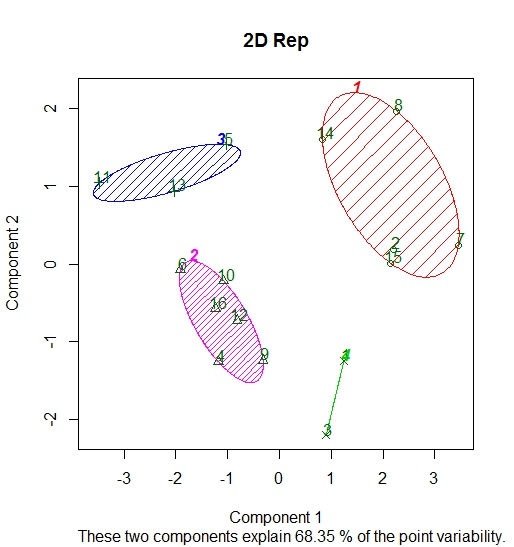
\includegraphics[width = .5\textwidth]{pictures/clustering/Kmeans.jpeg}
    \caption{K-means Clustering Method Result}
    \label{fig:Kmeans}
\end{figure}

\begin{figure}[htbp!]
    \centering
    \caption{Hierarchical Clustering Method Result}
    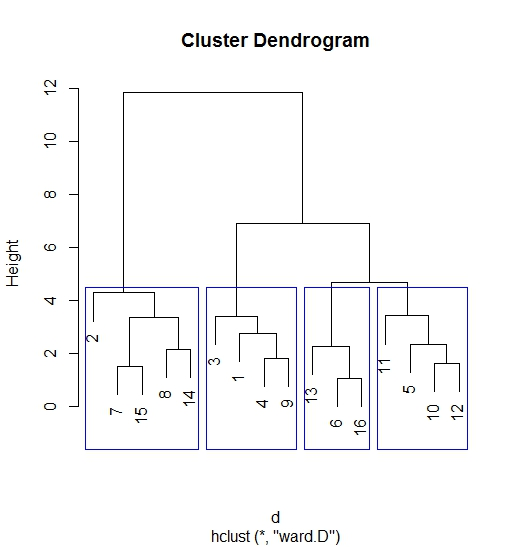
\includegraphics[width=0.5\textwidth]{pictures/clustering/Tree.jpeg}
    \label{fig:Tree}
\end{figure}

\section{Further Readings}

There are a wide variety of sources available that cover cluster analysis.
We recommend chapter 8 of \emph{Introduction to Data Mining} by Tan, Steinbach, and Kumar (2006).
The chapter can be fount at \url{https://www-users.cs.umn.edu/~kumar/dmbook/ch8.pdf}

Download the file located at \url{https://github.com/nosyarg/textbookdata/blob/master/berkeleyusdata.txt}.
